

\section{Data preparation}

%TODO add reference
The COMPAS dataset used in this study is publicly available through ProPublica's GitHub repository. This repository contains the dataset and other assets used by ProPublica to investigate the biases present in the COMPAS risk assessment tool.

The file chosen for this analysis is \textbf{\texttt{compas-scores-two-years.csv}}, as it provides the cleanest and most relevant data for general recidivism prediction. This CSV file contains the key data required for our study, including several attributes related to demographics, criminal history, COMPAS risk scores, and the two-year recidivism outcomes that are important for exploring the predictive capabilities and the ethical implications of machine learning models in the context of recidivism prediction. 

The dataset includes important information about individuals. Following an initial analysis, a list of the key fields in the dataset is below.

\begin{itemize}
	
	\item Personal Information, includes attributes such as \textbf{\texttt{age}}, \textbf{\texttt{race}}, \textbf{\texttt{age\_category}}, etc.
	
	\item Case and Event-Related Details are the fields prefixed with \textbf{\texttt{c\_}} that provide a timeline and details of a person's interactions with the criminal justice system.
	
	\item Violence Risk Assessment are the fields prefixed with \textbf{\texttt{v\_}} and are associated with the violence risk assessment in COMPAS. This dimension predicts violent recidivism risk.
	
	\item Case-Level Details for Violent Recidivism are the fields prefixed with \textbf{\texttt{vr\_}}. These fields provide additional details specific to violent recidivism events.
	
	\item Juvenile Criminal Record are the fields prefixed with \textbf{\texttt{juv\_}}. These fields capture information about an individual's juvenile criminal record, which is a key predictor of future adult criminal behaviour.
	
	\item Previous Charges and Severity can be deduced from fields such as \textbf{\texttt{priors\_count}} and \textbf{\texttt{juv\_}} fields.
	
	\item Additional fields, including \textbf{\texttt{r\_charge\_}}, \textbf{\texttt{r\_offense\_}}, \textbf{\texttt{vr\_}} fields, \textbf{\texttt{c\_charge\_degree}}, and \textbf{\texttt{c\_charge\_desc}}, provide a broader perspective on criminal history and severity.
	
	
	\item Two-Year Recidivism, or the \textbf{\texttt{two\_year\_recid}} field in the COMPAS dataset, indicates whether an individual reoffended (recidivated) within two years of their initial assessment or release. This field is critical for evaluating the predictive accuracy of the COMPAS risk assessment tool.
	
	\item Decile Score is a standardized risk score in the COMPAS dataset. It categorizes an individual's likelihood of recidivism into ten equal groups (deciles) where 1 is the lowest risk, and 10 is the highest risk. Each decile represents approximately 10\% of the sample when applied to a norm group.
	
\end{itemize}

%Suppose that we observe the following data:

%\begin{table}[!ht]
%	\centering
%	\begin{tabular}{|l|l|}
%		\hline
%		Field & Value \\ \hline
%		\textbf{\texttt{priors\_count}} & 5 \\ \hline
%		\textbf{\texttt{juv\_felony\_count}} & 2 \\ \hline
%		\textbf{\texttt{juv\_misdemeanor\_count}} & 3 \\ \hline
%		\textbf{\texttt{r\_charge\_degree}} & Felony \\ \hline
%	\end{tabular}
%\end{table}

%We can interpret this as an individual who has five total prior charges, including:

%\begin{itemize}
%	\item 2 juvenile felonies
%	\item 3 juvenile misdemeanours
%	\item The severity of previous charges includes felonies (\textbf{\texttt{r\_charge\_degree}}).
%\end{itemize}


\subsection{Preparing the data for further analysis and training}

Before we can perform any analysis or apply machine learning techniques, it is important to pre-process and prepare the dataset so that we can handle missing values, encode categorical features, and split the data into training, testing, and validation sets. This step will produce a clean dataset for building accurate and unbiased models. The following steps outline the procedures to prepare the dataset for further analysis and training.


\subsection{Initial look at data and missing values handling}

The dataset has 7214 instances over 53 columns. The COMPAS system risk factor is the field  \textbf{\texttt{decile\_score}}, but the dataset also contains information about whether or not the person recidivised through the label \textbf{\texttt{two\_year\_recid}}. 

The first step in this data analysis step was  removing the features irrelevant to this exercise or with over 50\% missing records. We removed all the COMPAS-administrative labels and additional recidivism information apart from \textbf{\texttt{two\_year\_recid}}, narrowing the dataset to 17 fields.

The difference between \textbf{\texttt{c\_jail\_in}} and \textbf{\texttt{c\_jail\_out}} was calculated into a new field, \textbf{\texttt{days\_in\_jail}} and the difference between \textbf{\texttt{in\_custody}} and \textbf{\texttt{out\_custody}}, in a new field, \textbf{\texttt{days\_in\_custody}}. We subsequently removed the features containing date information from the dataset, together with \textbf{\texttt{days\_in\_custody}}, as it contained no information. At this stage, the dataset contains thirteen features: eight numerical, four categorical, and one descriptive. It also contains two labels, decile\_score, which we will treat as the leading label in this exercise and \textbf{\texttt{two\_year\_recid}}, which we are keeping to compare the prediction power of our models to the original one.


\subsection{Imputation of missing data}

While examining the resultant dataset, we noticed that \textbf{\texttt{days\_b\_screening\_arrest}} has  6907 values that are not null. Whilst it is possible to eliminate the rows that contain the null values at this stage, we replaced the missing values using a KNN imputation technique by grouping the numeric values of this dataset so that we can calculate the missing values. We checked this process by plotting the distribution of \textbf{\texttt{days\_b\_screening\_arrest}} before and after imputation to see if any variations occurred.

\begin{figure}[H]
	\centering
	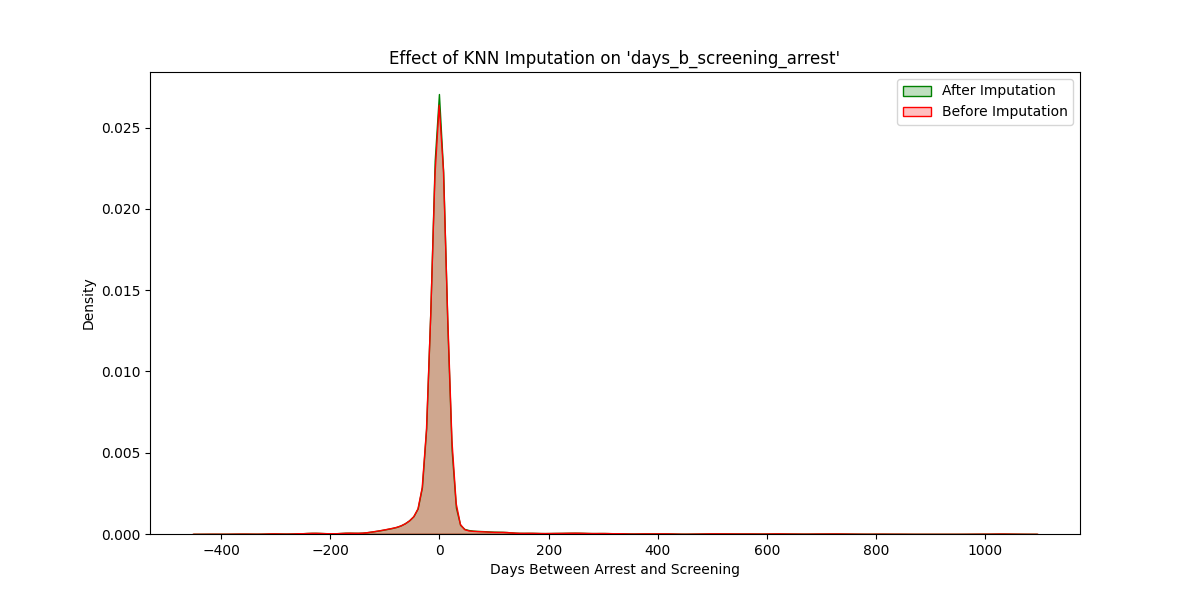
\includegraphics[width=0.9\linewidth]{img/imputation}
	\caption[Distribution \textbf{\texttt{days\_b\_screening\_arrest}} of before and after KNN imputation]{}
	\label{fig:imputation}
\end{figure}

At this stage, the dataset contains four categorical features that need encoding for machine learning algorithms. This section will focus on converting them into a numerical format using two encoding techniques. The categorical features and their values are listed below:

\begin{table}[!ht]
	\centering
	\begin{tabular}{|l|l|l|}
		\hline
		Feature & Description & Unique Values \\ \hline\hline
		\textbf{\texttt{sex}} & Gender of the individual & \shortstack{Male\\Female} \\ \hline
		\textbf{\texttt{race}} & Race of the individual & \shortstack[l]{African-American\\Caucasian\\Hispanic\\Asian\\Native American\\Other} \\ \hline
		\textbf{\texttt{age\_cat}} & Age category & \shortstack[l]{Less than 25\\25 - 45\\Greater than 45} \\ \hline
		\textbf{\texttt{c\_charge\_degree}} & \shortstack{Degree of the\\criminal charge} & \shortstack[l]{F (Felony)\\M (Misdemeanor)} \\ \hline
	\end{tabular}
\end{table}

The following transformations are applied:

\begin{itemize}[]
	\item One-Hot Encoding on \textbf{\texttt{sex}}, \textbf{\texttt{race}}, and \textbf{\texttt{c\_charge\_degree}}, transforming them into binary columns.
	\item Ordinal Encoding on \textbf{\texttt{age\_cat}}. This encoding technique was preferred over one-hot in this case as it preserves order, thus respecting the inherent ranking of the category.
\end{itemize}

The original categorical columns were retained in the dataset for future use in the analysis steps. 

\subsection{Splitting the data into train, test and dev}

A stratified shuffle split technique is preferred to create the train, test, and dev datasets whilst ensuring that the splits are proportional by \textbf{\texttt{race}}. In the first split, 80\% Train and 20\% Test are created, whilst in the Second split, The 20\% Test is further divided into 10\% Test and 10\% Dev.



	

	


	
	
	
	
	
	
	
	

	
	



